\section{Experiment}

\begin{frame}{Experiment: Adapting Algorithms to Finite Horizon}
\begin{itemize}
    \item Recall that we already know $\{V_0(s)\}_{s \in \mathcal{S}}$. We can use backtracking for evaluating any policy (Policy Iteration), or solve for the optimality operator (Value Iteration).
    \begin{align*}
    V_{t + 1}(s) = \sum_{p \in \mathcal{A}} \pi(p | s) \ \biggr[
    \sum_{s' > 0 \in \mathcal{S}} P(d = s - s' \mid p) \ \left\{ r(s, p, s') + \gamma V_t(s') \right\} \\
    + P(d \geq s \mid p) \left\{ r(s, p, 0) + \gamma V_t(0) \right\} \biggr]
    \end{align*}
    \item For Q-Learning and SARSA($\lambda$), we sample not just the initial state but also the initial timestep for generating the episodes. The timestep decreases with each transition, terminating in one of the absorbing states $\{V_0(s)\}_{s \in \mathcal{S}}$.
    \item For the step size, we use $\alpha = \ceil*{\frac{10}{m + 1}}$, borrowing from the paper Finite Horizon Q-learning by Vivek and Shalabh.
\end{itemize}
\end{frame}

\begin{frame}{Experiment: Hyperparameters}
\begin{center}
\begin{tabular}{|c|c|}
    \hline
    Hyperparameter & Value \\
    \hline
    Inventory (\#Seats) & 30 \\
    Booking Window (\#Days) & 30 \\
    Prices & $\{5000, 7500, 10000, 12500, 15000\}$ \\
    Discount Factor & 0.99 \\
    Epsilon & 1.00 \\
    Trace Decay & 0.90 \\
    Number of Episodes & 100,000 \\
    \hline
\end{tabular}
\end{center}
\end{frame}

\begin{frame}{Experiment: Value Function}
\begin{figure}
    \centering
    \begin{subfigure}{\textwidth}
        \centering
        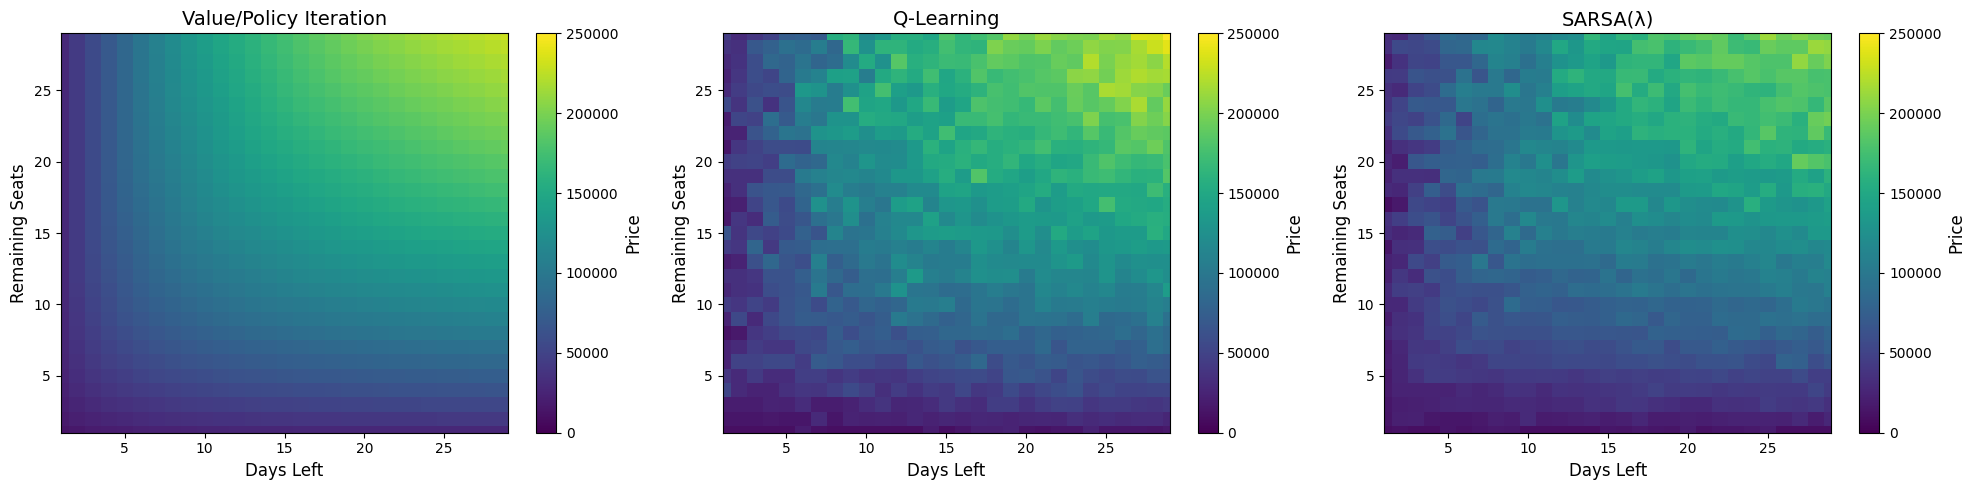
\includegraphics[width=\textwidth]{value_function.png}
        \caption{Original Values}
    \end{subfigure}
    \begin{subfigure}{\textwidth}
        \centering
        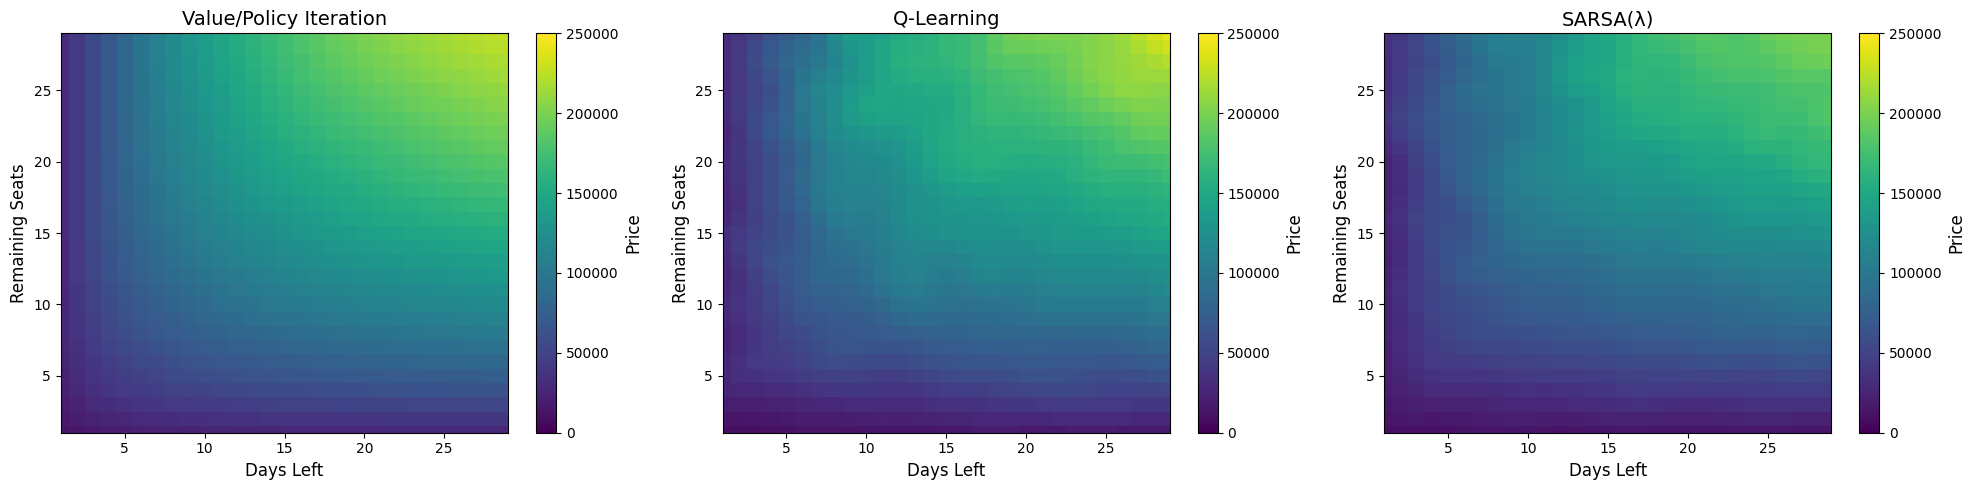
\includegraphics[width=\textwidth]{value_function_smooth.png}
        \caption{Gaussian Filtered ($\sigma = 1$) \footnote{Equivalent to averaging in a $3 \times 3$ window.}}
    \end{subfigure}
    \caption{Value function learned by different algorithms.}
\end{figure}
\end{frame}

\begin{frame}{Experiment: Learned Policies}
\begin{figure}
    \centering
    \begin{subfigure}{\textwidth}
        \centering
        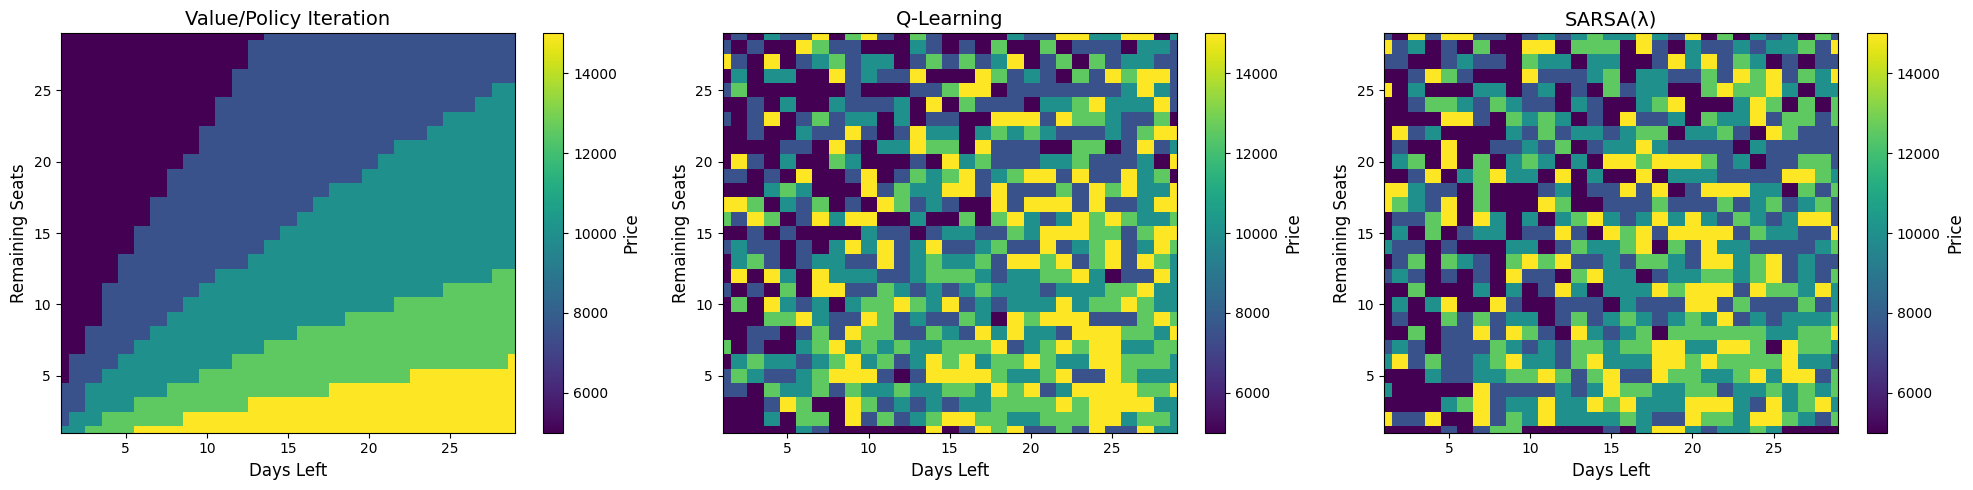
\includegraphics[width=\textwidth]{policy.png}
        \caption{Original Policy}
    \end{subfigure}
    \begin{subfigure}{\textwidth}
        \centering
        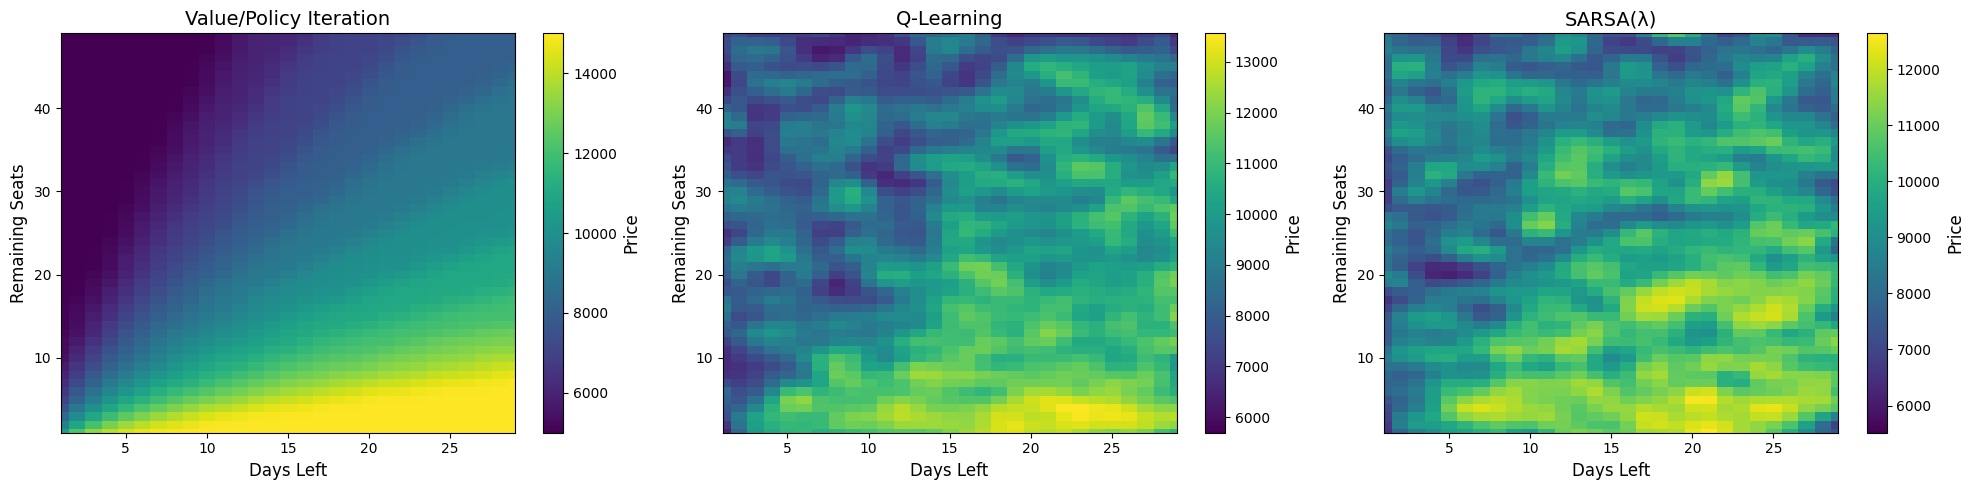
\includegraphics[width=\textwidth]{policy_smooth.png}
        \caption{Gaussian Filtered ($\sigma = 1$)}
    \end{subfigure}
    \caption{Policy learned by different algorithms.}
\end{figure}
\end{frame}


\begin{frame}{Experiment: Simulation of Different Policies}
\begin{figure}
    \centering
    \begin{subfigure}{0.45\textwidth}
        \centering
        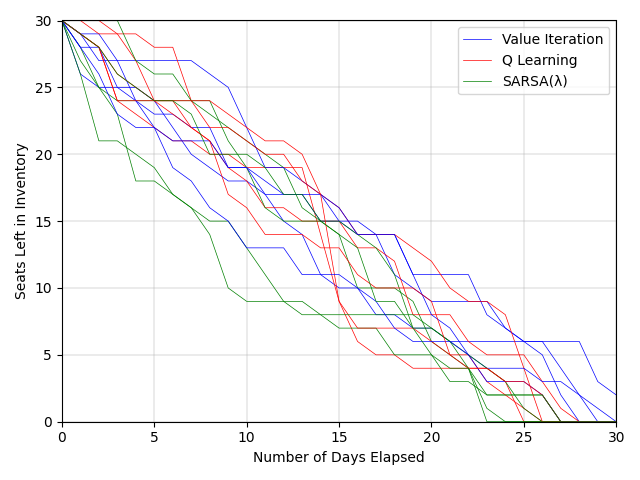
\includegraphics[width=\textwidth]{trajectory_1.png}
        \caption{Individual Trajectories}
    \end{subfigure}
    \begin{subfigure}{0.45\textwidth}
        \centering
        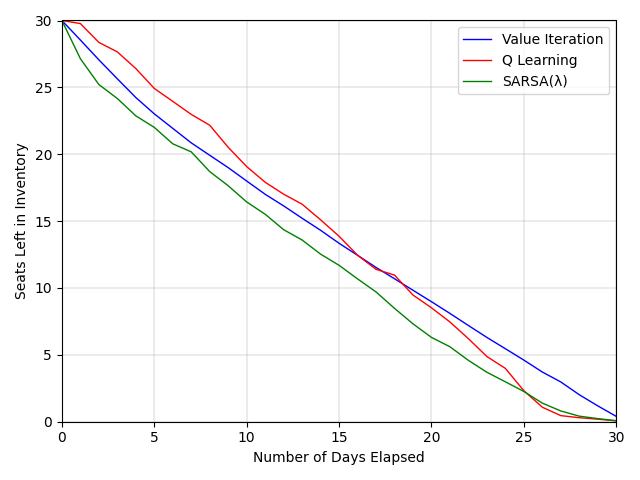
\includegraphics[width=\textwidth]{average_trajectory.png}
        \caption{Average Trajectory}
    \end{subfigure}
    \caption{Trajectory of independent simulations.}
\end{figure}
\end{frame}

\begin{frame}{Experiment: Trends in Value Function}
\begin{figure}
    \centering
    \begin{subfigure}{0.35\textwidth}
        \centering
        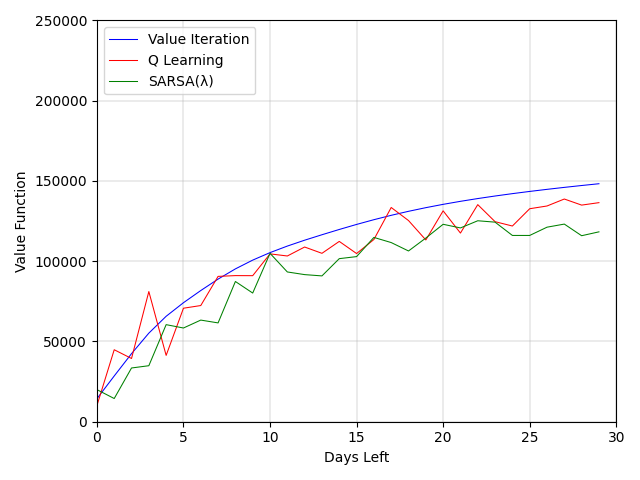
\includegraphics[width=\textwidth]{inventory_15.png}
        \caption{Fixed Inventory (k=15)}
    \end{subfigure}
    \begin{subfigure}{0.35\textwidth}
        \centering
        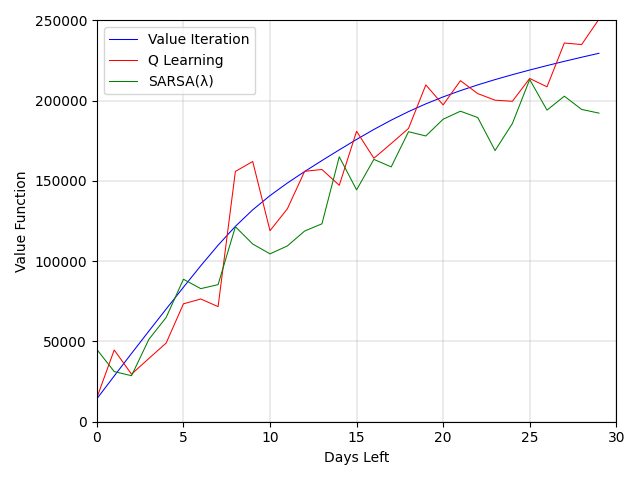
\includegraphics[width=\textwidth]{inventory_30.png}
        \caption{Fixed Inventory (k=30)}
    \end{subfigure}
    \begin{subfigure}{0.35\textwidth}
        \centering
        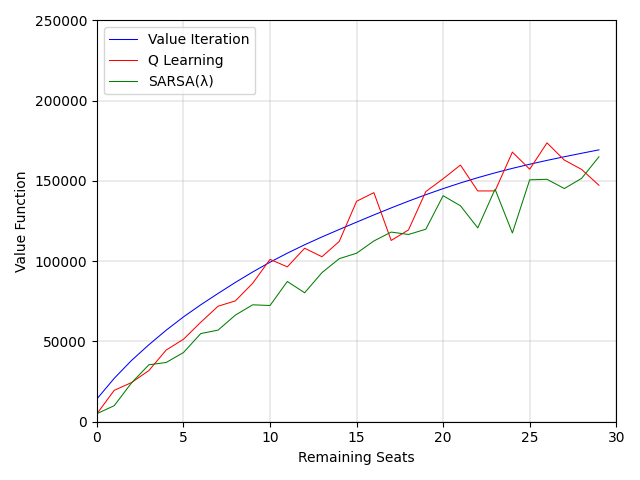
\includegraphics[width=\textwidth]{timestep_15.png}
        \caption{Fixed Timestep (t=15)}
    \end{subfigure}
    \begin{subfigure}{0.35\textwidth}
        \centering
        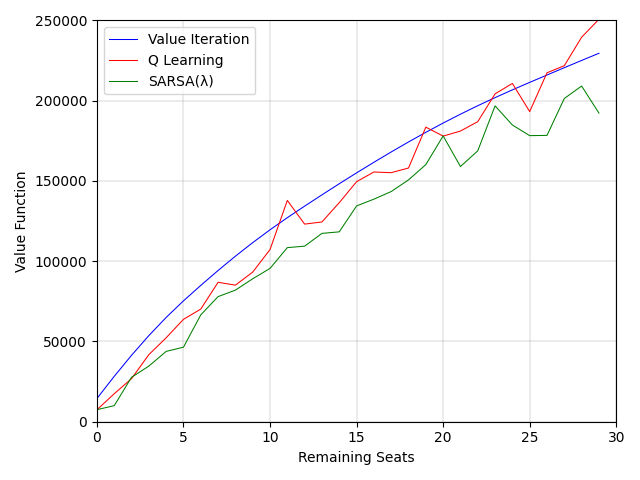
\includegraphics[width=\textwidth]{timestep_30.png}
        \caption{Fixed Timestep (t=30)}
    \end{subfigure}
    \caption{Variation in value function with inventory and timestep.}
\end{figure}
\end{frame}

\begin{frame}{Experiment: Trends in State Value Function}
\begin{figure}
    \centering
    \begin{subfigure}{0.35\textwidth}
        \centering
        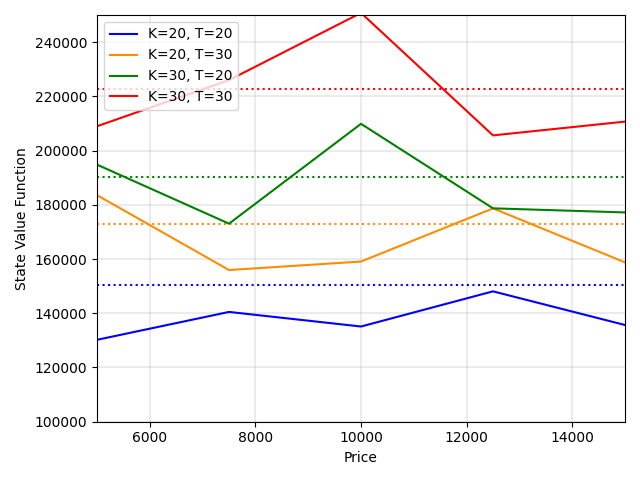
\includegraphics[width=\textwidth]{state_action_ql.png}
        \caption{Q-Learning}
    \end{subfigure}
    \begin{subfigure}{0.35\textwidth}
        \centering
        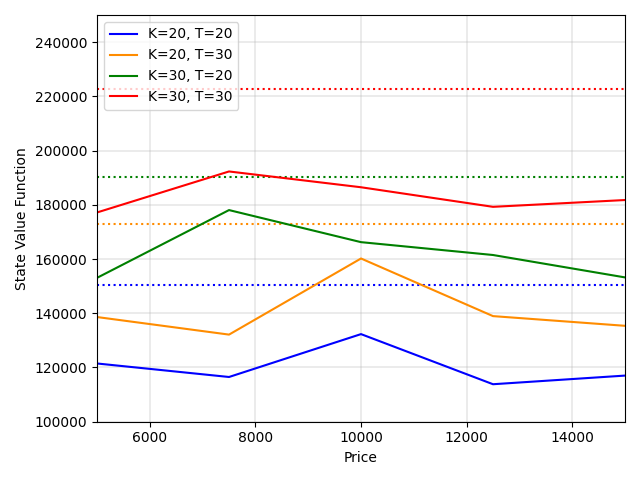
\includegraphics[width=\textwidth]{state_action_sarsa.png}
        \caption{SARSA($\lambda$)}
    \end{subfigure}
    \caption{Variation in state value function for different prices. The dotted line represents the true value function (learned by VI/PI) for the optimal price.}
\end{figure}
\end{frame}

\begin{frame}{Experiment: Evolution of Rewards and Regrets}
\begin{figure}
    \centering
    \begin{subfigure}{\textwidth}
        \centering
        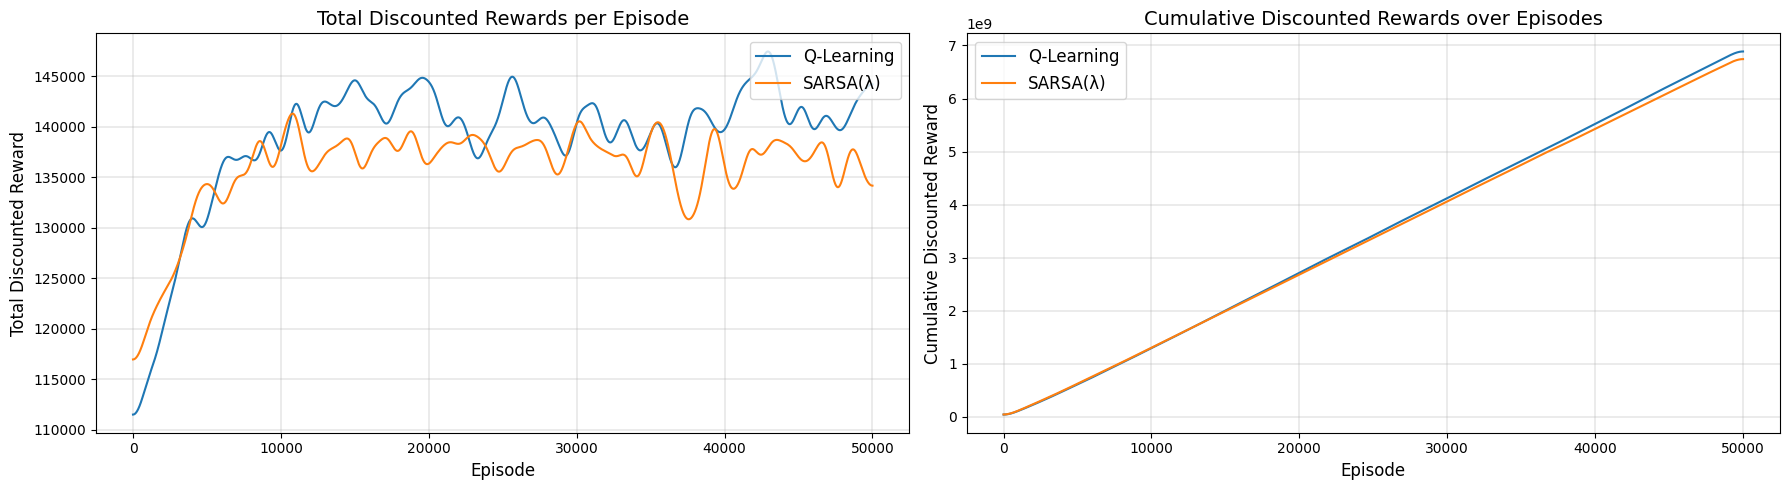
\includegraphics[width=0.9\textwidth]{reward.png}
        \caption{Episodic and Cumulative Rewards}
    \end{subfigure}
    \begin{subfigure}{\textwidth}
        \centering
        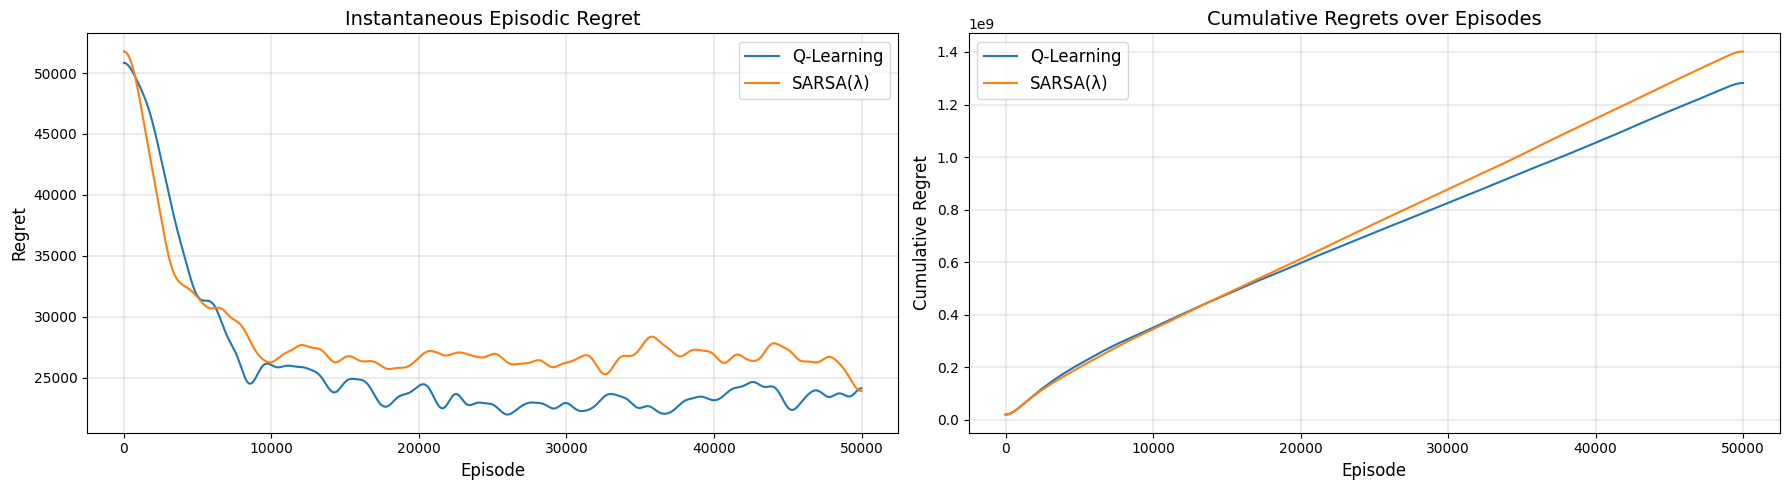
\includegraphics[width=0.9\textwidth]{regret.png}
        \caption{Episodic and Cumulative Regrets \footnote{All episodic metrics in the presentation are Gaussian Filtered with $\sigma = 500$, equivalent to averaging over 2000 entries.}}
    \end{subfigure}
    \caption{Rewards and regrets incurred by different algorithms.}
\end{figure}
\end{frame}

\begin{frame}{Experiment: Evolution of Policy and Value Function}
\begin{figure}
    \centering
    \begin{subfigure}{\textwidth}
        \centering
        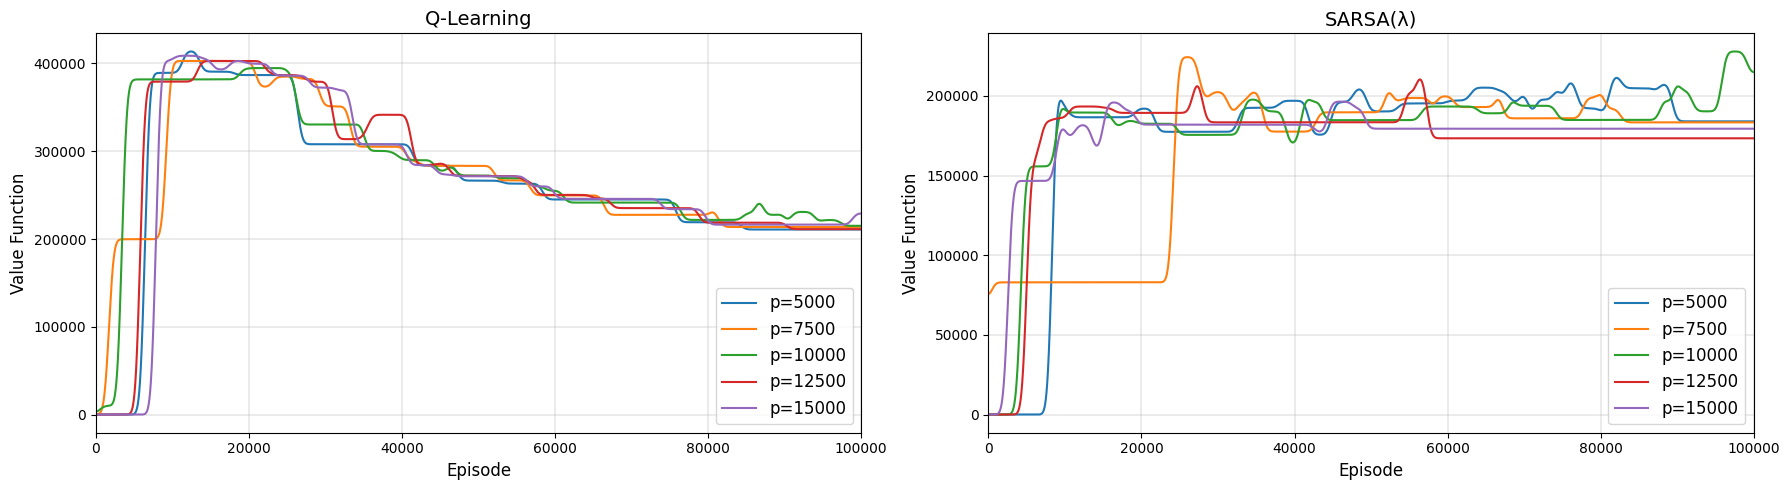
\includegraphics[width=0.9\textwidth]{value_evolution.png}
        \caption{State Value Function}
    \end{subfigure}
    \begin{subfigure}{\textwidth}
        \centering
        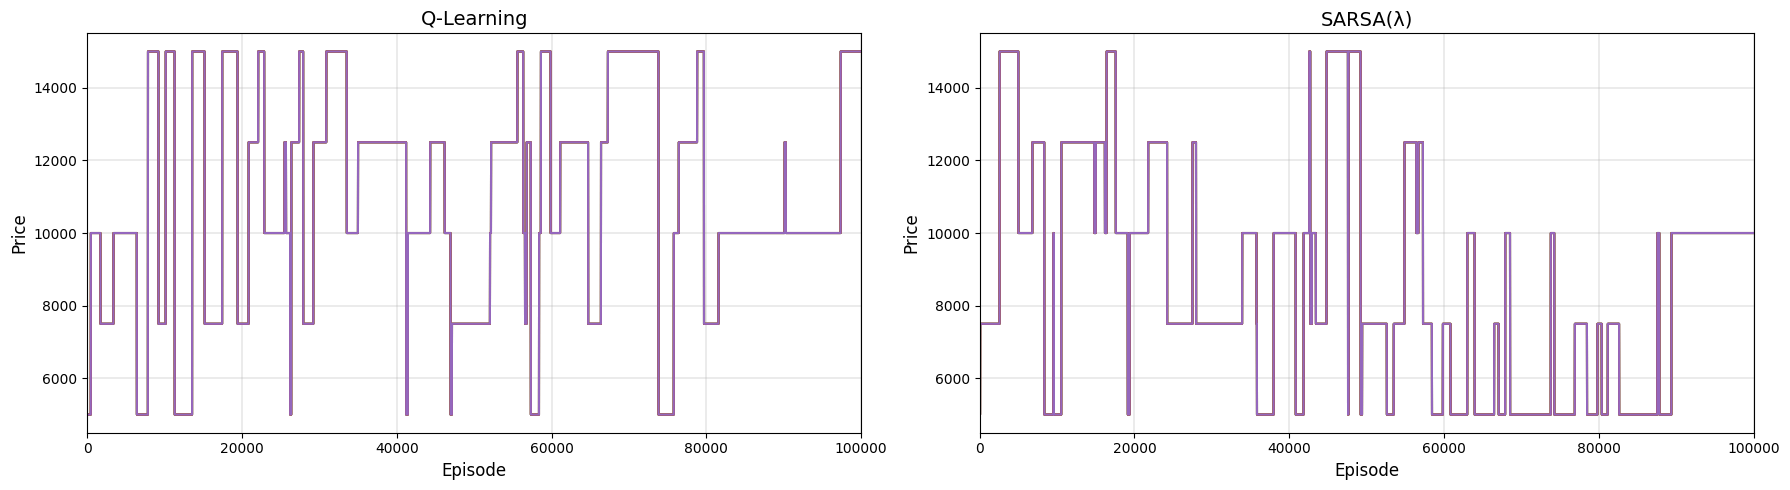
\includegraphics[width=0.9\textwidth]{policy_evolution.png}
        \caption{Learned Policy}
    \end{subfigure}
    \caption{Evolution of policy and state value function for a fixed state and time (k=30, t=30).}
\end{figure}
\end{frame}
